\FloatBarrier
\section{Pole placement}
The Matlab implementation of the original system's transfer function is given in \autoref{code:pp01}. Its step response, shown in \autoref{fig:pp01}, indicates that the original system is unstable.

\begin{code}
	\begin{matlabcode}{firstnumber = 12}
s = tf('s');
G_Original = ((5*((0.7*s)+1)*(s+0.8))/((((3*s)+1)^2)*((2*s)-1)));
if drawPlot
	figure;
	step(G_Original, 'b');
	legend('Step response');
	title('Step Response of Original System');
	fontsize( 24 ,"points");
end
	\end{matlabcode}
	\captionof{listing}{Original system}
	\label{code:pp01}
\end{code}

\begin{figure}
	\centering
	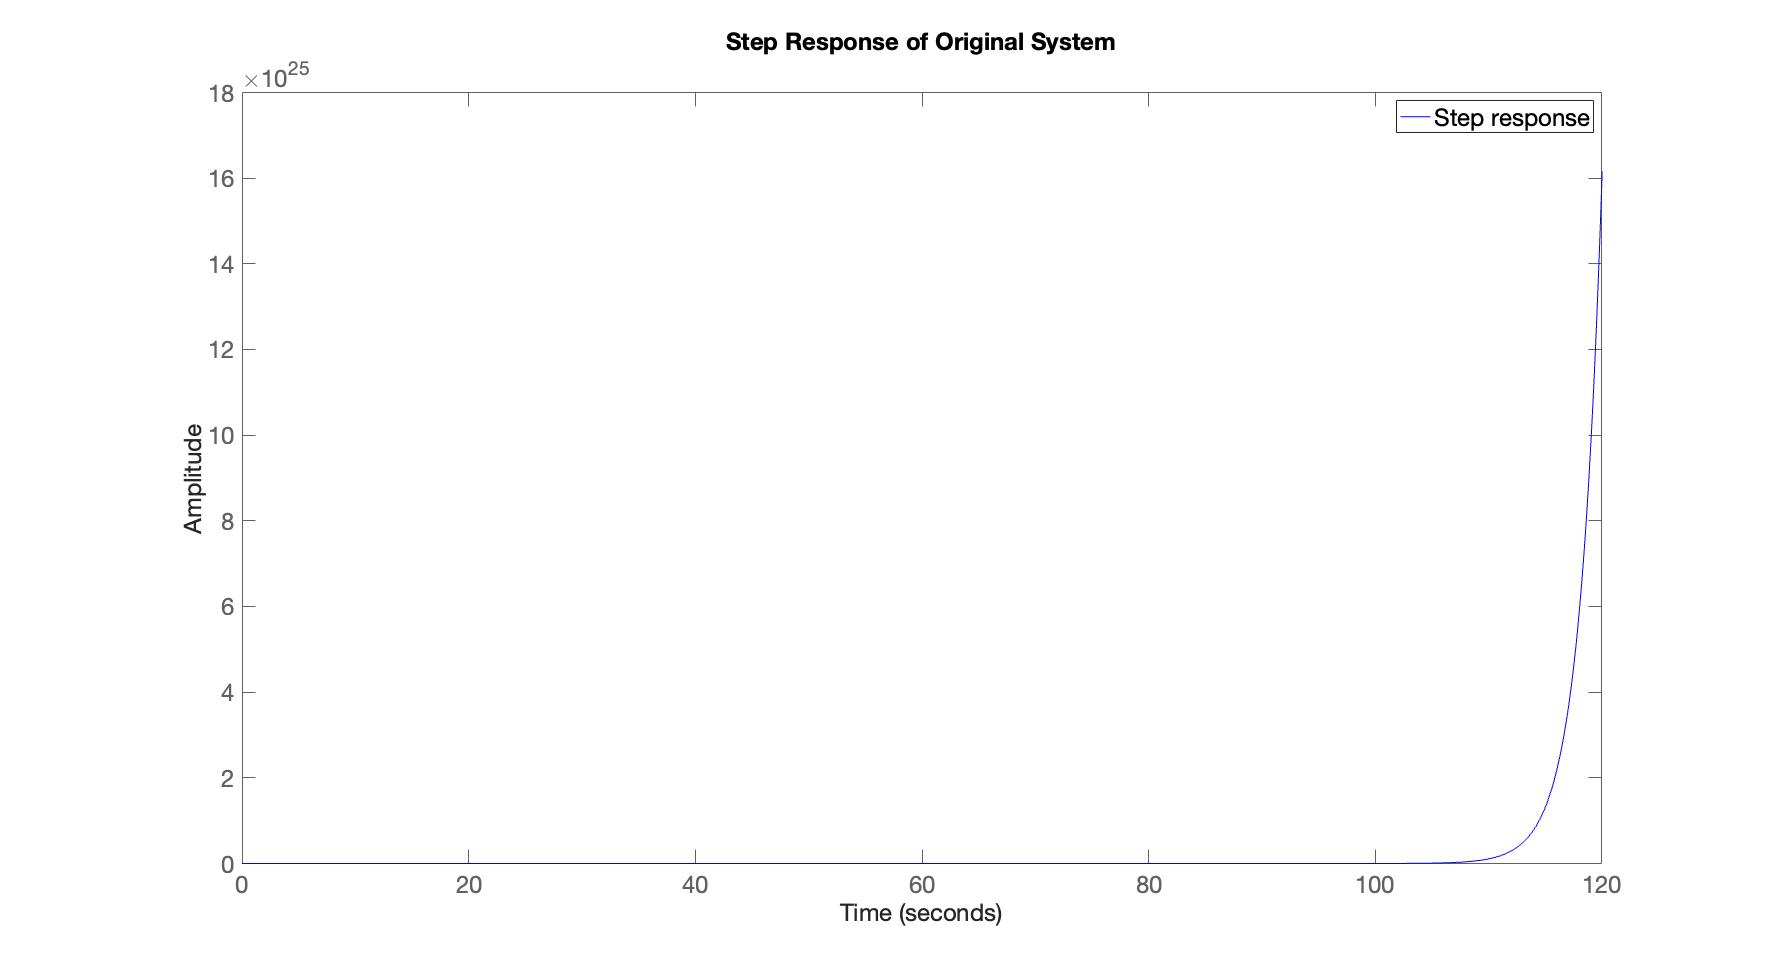
\includegraphics[width=\textwidth]{images/pp01.png}
	\caption{Original system step response}
	\label{fig:pp01}
\end{figure}

To enable the calculation of the system's settling time, the unstable pole was mirrored and the system was discretized, as implemented in the code shown in \autoref{code:pp02}. The step response of the resulting, modified system is presented in \autoref{fig:pp02}.

\begin{code}
	\begin{matlabcode}{firstnumber = 56}
%% Discrete transfer function of stable transfer function
G_discrete = c2d(G, sampleTimeIntervals, 'zoh');
% Compare step responses
if drawPlot
	figure;
	step(G, 'b');
	hold on;
	step(G_discrete, 'r');
	legend('Continuous', 'Discrete');
	title('Step Response Comparison');
	fontsize( 24 ,"points");
end
	\end{matlabcode}
	\captionof{listing}{Discrete stable system}
	\label{code:pp02}
\end{code}

\begin{figure}
	\centering
	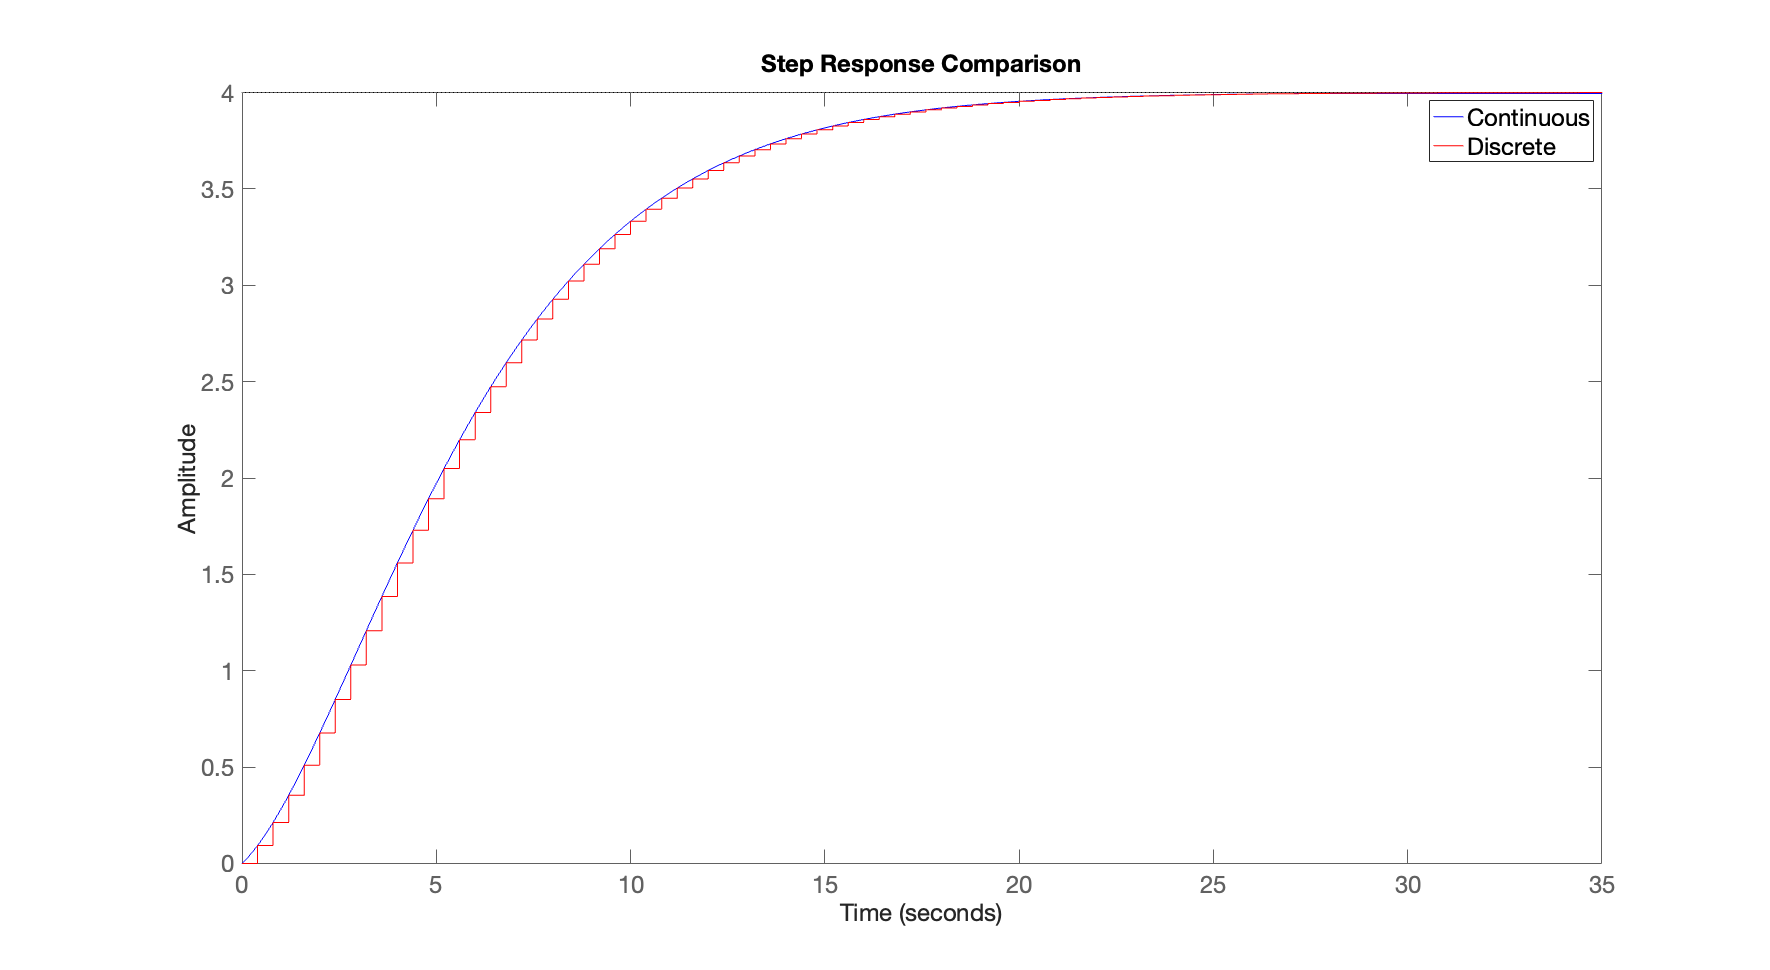
\includegraphics[width=\textwidth]{images/pp02.png}
	\caption{Discrete \& contineus stable system step response}
	\label{fig:pp02}
\end{figure}

Additionally, we generated the pulse train required for subsequent sections. We then evaluated various pulse periods and widths to determine the required configuration based on the resulting settling time. The code for generating these pulses is depicted in \autoref{code:pp03}, while \autoref{fig:pp03} presents the stable system's output responses to each corresponding pulse input.

\begin{code}
	\begin{matlabcode}{firstnumber = 70}
k = 5; % 4x settling time
Tp_min = k * Ts; % Minimum recommended period between pulses

fprintf('Minimum Recommended Pulse Period (Tp): %.2f seconds\n', Tp_min);

%Simulation Time
Tsim = 20 * Tp_min; 
t = 0:sampleTimeIntervals:Tsim;

%Pulse Train 1 (Respecting Settling Time)
u1 = gensig('square' ,Tp_min , Tsim , Gz.Ts); 
u2 = gensig('square' ,Tp_min/k , Tsim , Gz.Ts); 

y1 = lsim(G_discrete, u1, t);
y2 = lsim(G_discrete, u2, t);

if drawPlot
	figure;
	subplot(2,1,1);
	plot(t, u1, 'r-', t, y1, 'b-');fontsize( 24 ,"points");
	title(sprintf('Response with fpulse Allows Settling '));
	xlabel('Time (s)'); ylabel('Amplitude'); legend('Input Pulse', 'System Output'); grid on;
	ylim([-0.1 4.5]); 
	
	subplot(2,1,2);
	plot(t, u2, 'r-', t, y2, 'b-');fontsize( 24 ,"points");
	title(sprintf('Response with fpulse Too Fast'));
	xlabel('Time (s)'); ylabel('Amplitude'); legend('Input Pulse', 'System Output'); grid on;
	ylim([-0.1 4.5]);  
end
	\end{matlabcode}
	\captionof{listing}{Discrete stable system}
	\label{code:pp03}
\end{code}

\begin{figure}
	\centering
	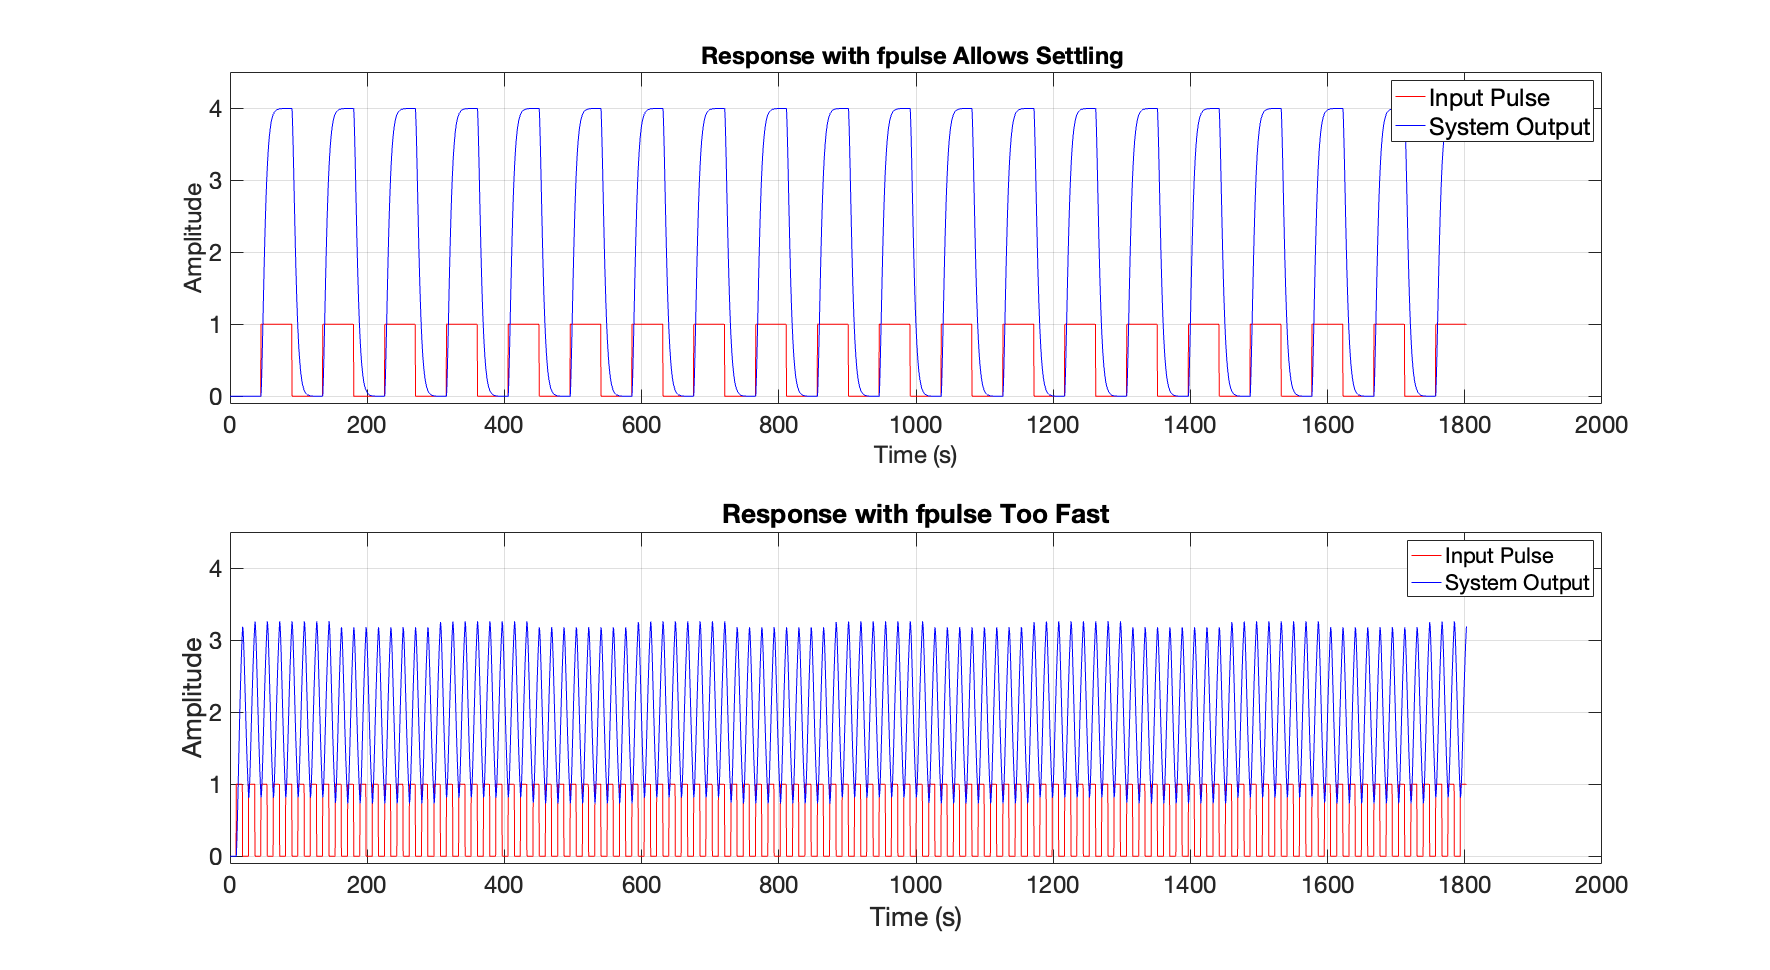
\includegraphics[width=\textwidth]{images/pp03.png}
	\caption{Pulse input and response}
	\label{fig:pp03}
\end{figure}

\noindent The code for this section is available at \lstinline|assignment2/part1/PP1_0.m|. 


\import{Part1Subsections/}{q1.tex}
\import{Part1Subsections/}{q2.tex}
\import{Part1Subsections/}{q3.tex}
\import{Part1Subsections/}{q4.tex}